%============================================================
%  Capitolo 1 – Architetture di Base
%============================================================
\chapter{Architetture di Base}
\label{ch:basic-arch}

Questo capitolo introduce i moduli fondamentali che estendono le reti neurali
standard con operazioni moltiplicative e meccanismi di condivisione dei
parametri. Questi concetti sono alla base di architetture moderne quali le reti
convoluzionali, i meccanismi di attenzione e i modelli Mixture of Experts
\citep{bishop2024, lecun2021}.

%------------------------------------------------------------
\section{Moduli Moltiplicativi}
\label{sec:multiplicative}

Le reti neurali classiche calcolano combinazioni lineari degli ingressi seguite
da una non-linearità. I \textbf{moduli moltiplicativi} generalizzano questa
idea permettendo che i pesi stessi dipendano da un secondo ingresso,
introducendo interazioni di ordine superiore tra feature.

\subsection{Unità Sigma-Pi e layer quadratico}

\begin{definizione}[Unità Sigma-Pi]
In una rete standard il pre-input è $s_i = \sum_j w_{ij}\, x_j$.
Nelle \textbf{unità Sigma-Pi} i pesi dipendono linearmente da un secondo
vettore di ingresso $\vect{z}$:
\begin{equation}
  w_{ij} = \sum_k u_{ijk}\, z_k
  \quad\Longrightarrow\quad
  s_i = \sum_{j,k} u_{ijk}\, z_k\, x_j
\end{equation}
dove $u_{ijk}$ sono i parametri effettivi del modello.
\end{definizione}

L'operazione è bilineare: lineare in $\vect{z}$ e in $\vect{x}$, ma quadratica
nel vettore congiunto $(\vect{z}, \vect{x})$. La figura seguente mostra il
diagramma computazionale dell'unità Sigma-Pi e, a destra, il modulo di
attenzione come caso speciale \refbishop{6}.

\begin{figure}[H]
  \centering
  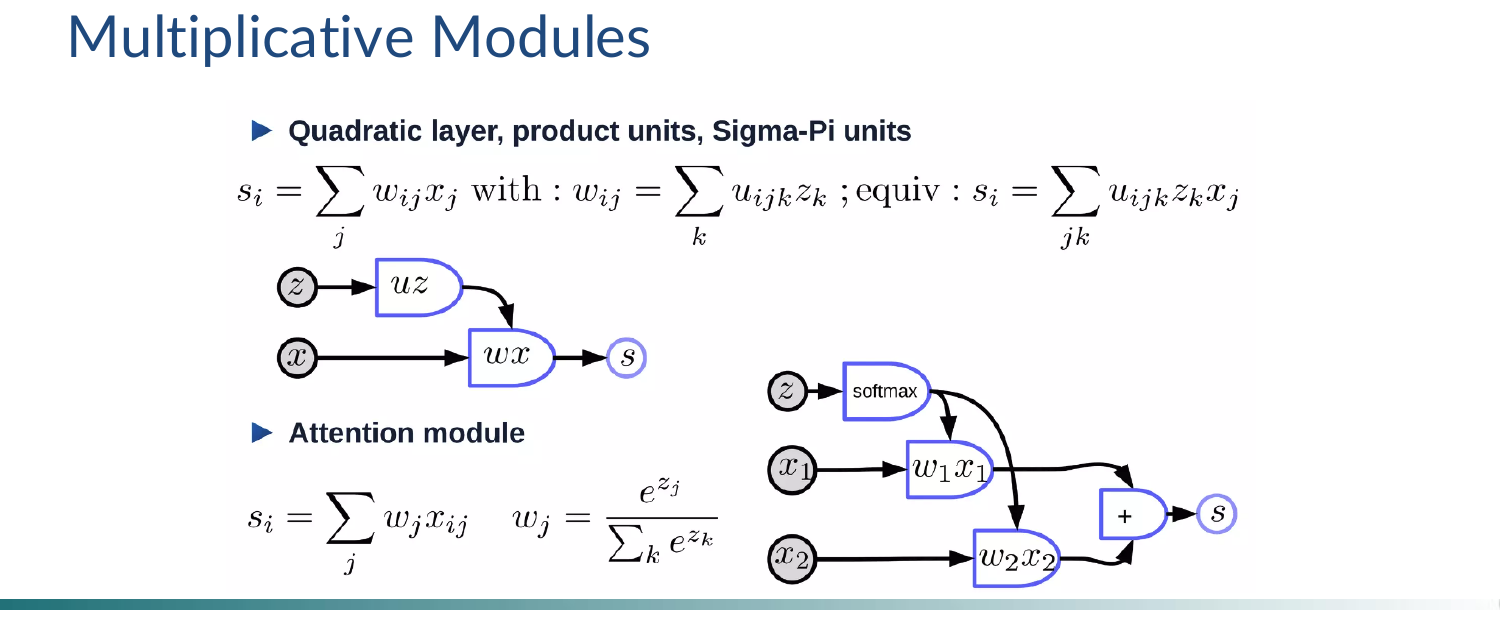
\includegraphics[width=0.88\linewidth]{figures/sigma_pi.png}
  \caption{Sinistra: unità Sigma-Pi -- il blocco $uz$ calcola i pesi dinamici
           da $z$, che vengono applicati all'ingresso $x$ nel blocco $wx$.
           Destra: modulo di attenzione -- $z$ passa per una softmax che
           produce i pesi $w_1, w_2$ per sommare le uscite pesate degli
           ingressi $x_1, x_2$.}
  \label{fig:sigma_pi}
\end{figure}

\subsection{Modulo di attenzione}

Il \textbf{meccanismo di attenzione} è il caso speciale in cui i pesi sono
normalizzati tramite softmax, formando una distribuzione di probabilità:
\begin{equation}
  s_i = \sum_j w_j\, x_{ij}, \qquad
  w_j = \frac{e^{z_j}}{\sum_k e^{z_k}} = \softmax(\vect{z})_j.
\end{equation}
La rete sceglie dinamicamente su quale ingresso concentrarsi in base al
contesto $\vect{z}$. Nel corso NYU \citep{lecun2021}, l'attenzione è
interpretata come un meccanismo di \textit{recupero soft} da una memoria
associativa, che anticipa direttamente l'architettura Transformer
\citep{vaswani2017}.

\subsection{Proprietà di differenziabilità}

Il modulo moltiplicativo con selezione discreta ($z_1 \in \{0,1\}$) non è
differenziabile rispetto ai parametri della porta di controllo, ma rimane
differenziabile rispetto a ingressi e uscite. La corrispondenza con la
selezione matriciale è:
\begin{equation}
  z_1{=}1,\,z_2{=}0:\;
  \begin{bmatrix}1&0\end{bmatrix}\!\begin{pmatrix}x_1\\x_2\end{pmatrix}=x_1,
  \quad
  z_1{=}0,\,z_2{=}1:\;
  \begin{bmatrix}0&1\end{bmatrix}\!\begin{pmatrix}x_1\\x_2\end{pmatrix}=x_2.
\end{equation}

\begin{figure}[H]
  \centering
  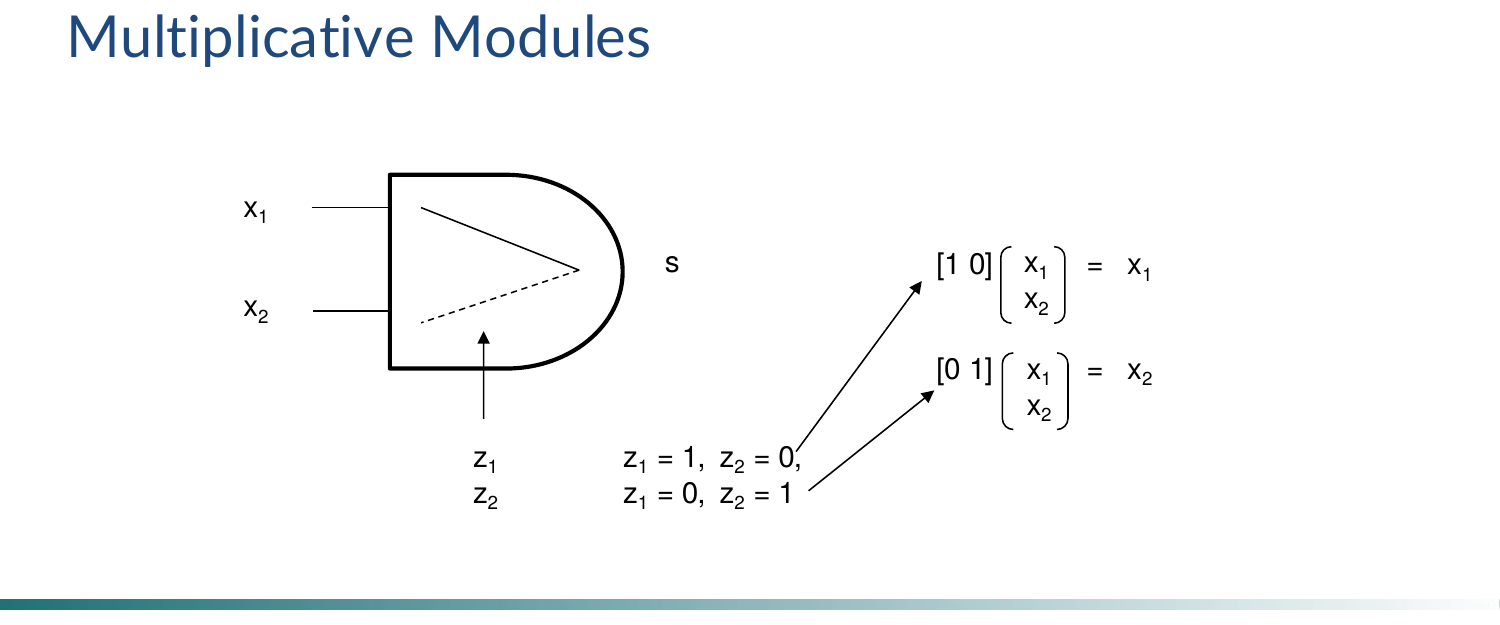
\includegraphics[width=0.72\linewidth]{figures/mux_discrete.png}
  \caption{Selezione discreta: quando $z_1=1, z_2=0$ il modulo seleziona
           $x_1$; quando $z_1=0, z_2=1$ seleziona $x_2$.}
  \label{fig:mux_discrete}
\end{figure}

\begin{figure}[H]
  \centering
  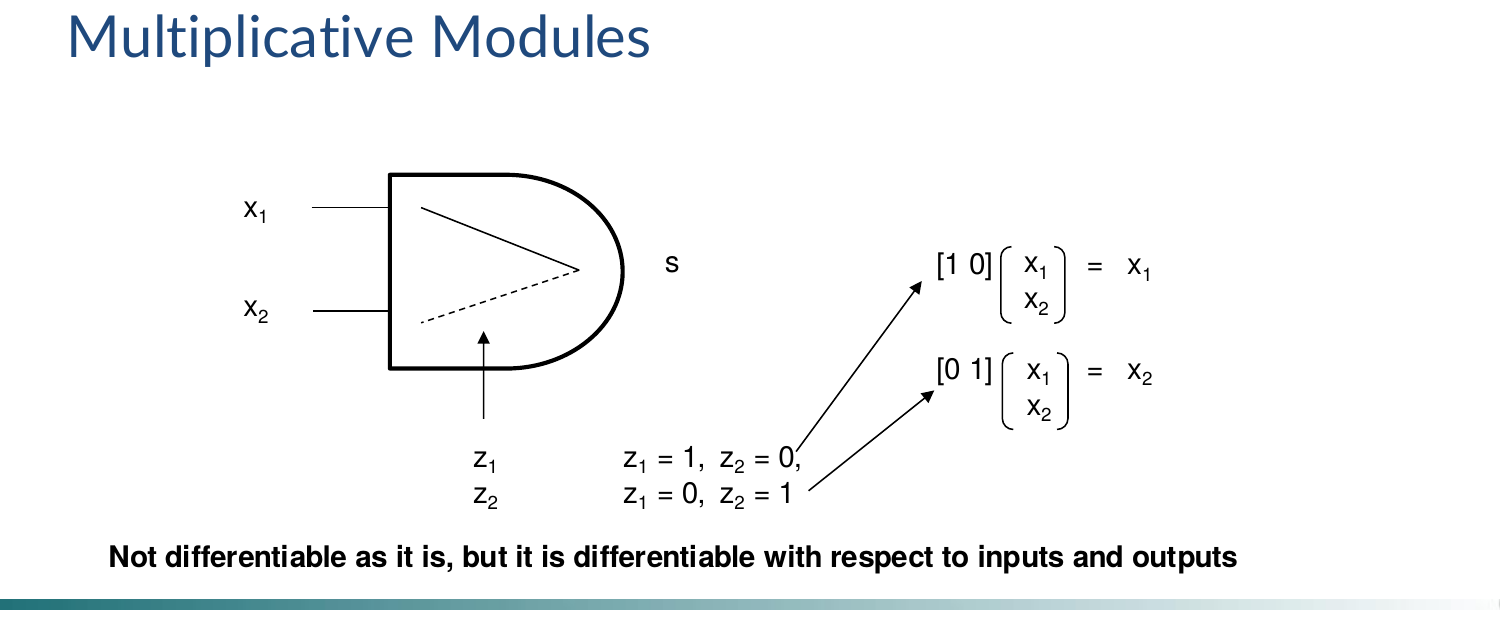
\includegraphics[width=0.72\linewidth]{figures/mux_diff.png}
  \caption{Il modulo con selezione discreta non è differenziabile come tale,
           ma lo è rispetto agli ingressi e alle uscite: il rilassamento
           tramite softmax rende tutto addestrabile con backpropagation.}
  \label{fig:mux_diff}
\end{figure}

%------------------------------------------------------------
\section{Mixture of Experts}
\label{sec:moe}

Il \textbf{Mixture of Experts} (MoE) generalizza il modulo di attenzione
applicandolo a intere reti esperto \citep{jacobs1991}:
\begin{equation}
  s_i = \sum_j w_j\, x_{ij}, \qquad
  w_j = \softmax(\vect{z})_j.
\end{equation}

\begin{figure}[H]
  \centering
  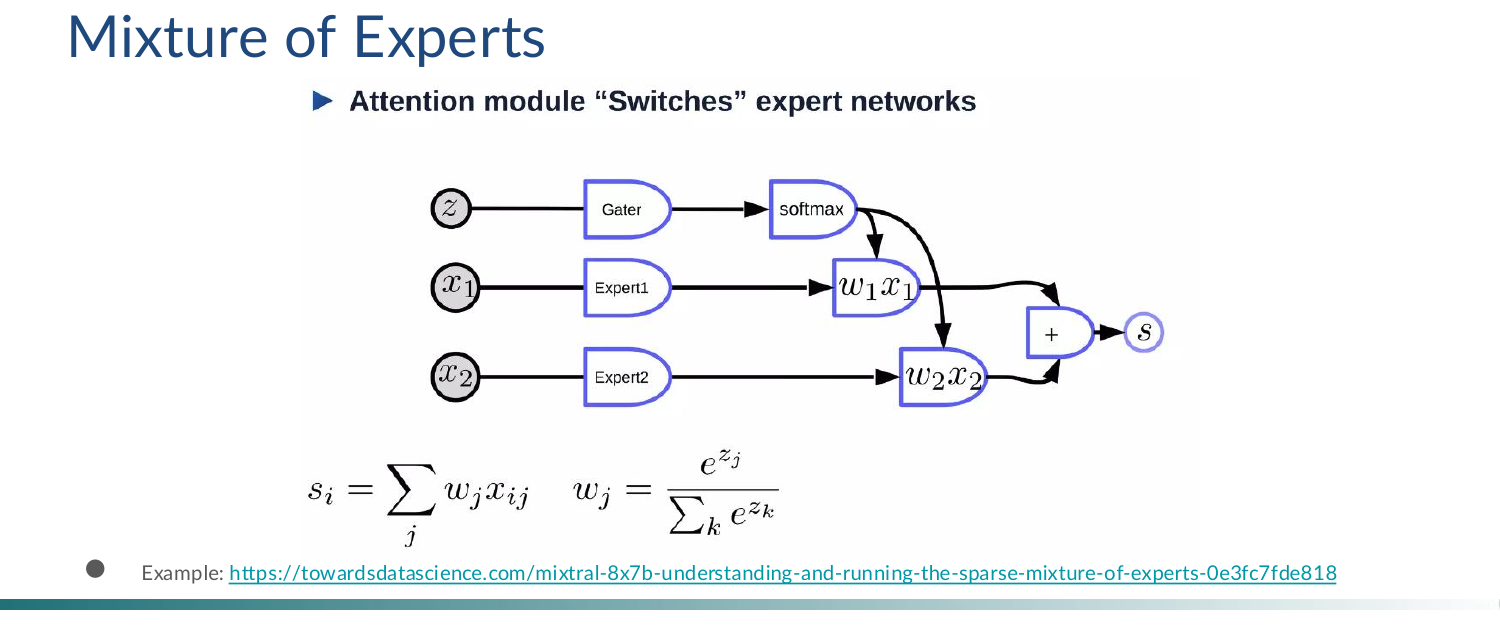
\includegraphics[width=0.82\linewidth]{figures/moe.png}
  \caption{Mixture of Experts: la rete Gater produce i pesi softmax a partire
           da $z$; Expert1 e Expert2 elaborano $x_1$ e $x_2$; le loro uscite
           pesate vengono sommate per produrre $s$.}
  \label{fig:moe}
\end{figure}

Nelle architetture moderne come \textbf{Mixtral 8$\times$7B}
\citep{mixtral2023}, il gating è \textit{sparse}: per ogni token vengono
attivati solo $k$ esperti su $n$ (tipicamente $k{=}2$ su $n{=}8$), con
\textit{top-k routing}. Questo garantisce alta capacità parametrica a basso
costo computazionale, ma introduce la sfida del \textit{load balancing}.

%------------------------------------------------------------
\section{Trasformazioni dei Parametri}
\label{sec:param-transform}

Dato il vettore di parametri interno $\vect{u}$, i pesi operativi $\vect{w}$
sono ottenuti tramite una funzione differenziabile $H$:
\begin{equation}
  \vect{w} = H(\vect{u}).
\end{equation}
Applicando la regola della catena con learning rate $\eta$:
\begin{align}
  u &\leftarrow u - \eta\, \pd{H^T}{u}\, \pd{C^T}{w} \\
  w &\leftarrow w - \eta\, \pd{H}{u}\, \pd{H^T}{u}\, \pd{C^T}{w}
\end{align}
con Jacobiane di dimensioni $[N_u \times N_w]$, $[N_w \times N_u]$,
$[N_w \times 1]$.

\begin{figure}[H]
  \centering
  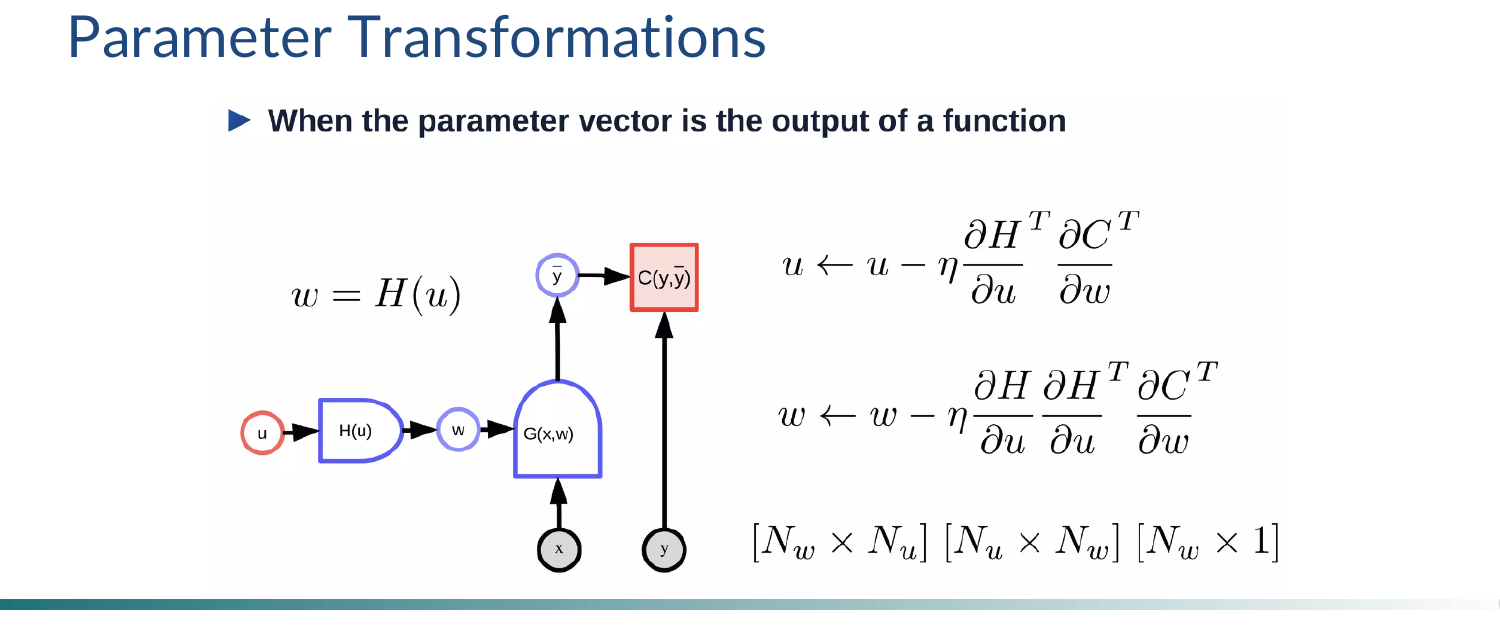
\includegraphics[width=0.82\linewidth]{figures/param_transform.png}
  \caption{Schema della trasformazione parametrica: $u$ passa per $H(u)$
           per produrre $w$, che viene usato in $G(x,w)$. Il backward
           richiede la Jacobiana di $H$ sia rispetto a $u$ sia rispetto a $w$.}
  \label{fig:param_transform}
\end{figure}

\subsection{Weight sharing -- condivisione dei pesi}

Il caso più importante è il \textbf{weight sharing}: $H(\vect{u})$ replica
alcune componenti di $\vect{u}$ in più componenti di $\vect{w}$, ad esempio
$w_1 = w_2 = u_1$, $w_3 = w_4 = u_2$. In backpropagation i gradienti di
tutte le copie vengono \textbf{sommati}:
\begin{equation}
  \pd{C}{u_k} = \sum_{j=1}^{m} \pd{C}{w_{i_j}}.
\end{equation}

\begin{figure}[H]
  \centering
  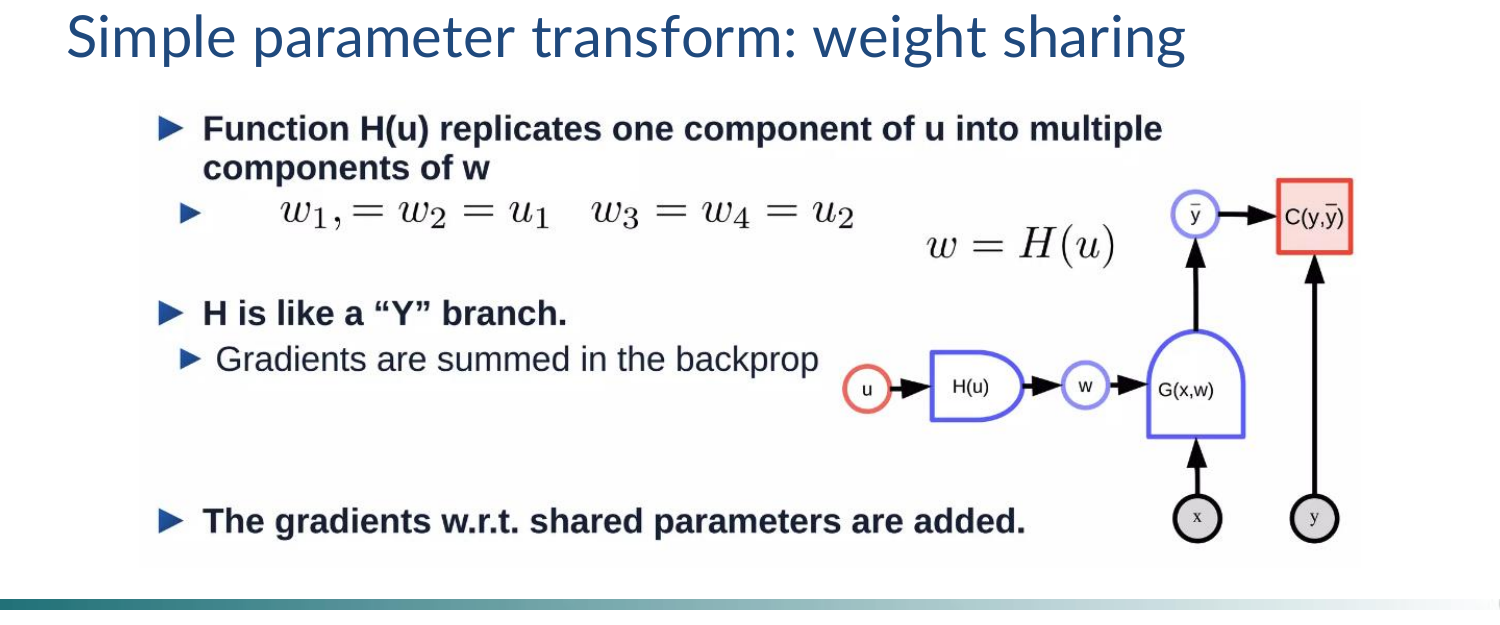
\includegraphics[width=0.82\linewidth]{figures/weight_sharing.png}
  \caption{Weight sharing: $H(u)$ si comporta come un ``ramo Y'', replicando
           il parametro $u_1$ nei pesi $w_1=w_2$ e $u_2$ nei pesi $w_3=w_4$.
           I gradienti w.r.t.\ i parametri condivisi vengono sommati.}
  \label{fig:weight_sharing}
\end{figure}

\subsection{Shared weights per la rilevazione di motif}

Applicando lo stesso $\vect{w}$ a finestre diverse dell'input e raccogliendo
con MAX pooling, si ottiene un rilevatore di motif invariante per traslazione.
Questo schema è esattamente una \textit{convoluzione 1D} seguita da global
max-pooling \citep{lecun1998}.

\begin{figure}[H]
  \centering
  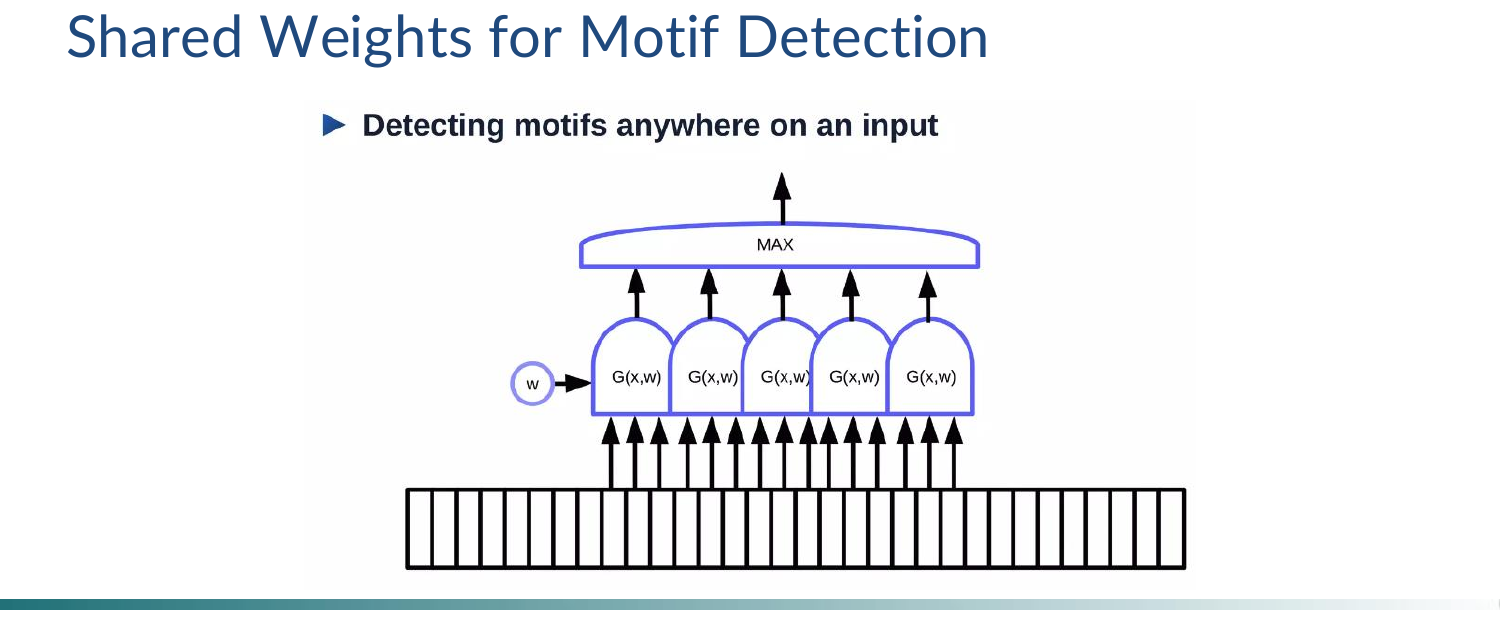
\includegraphics[width=0.82\linewidth]{figures/motif.png}
  \caption{Rilevazione di motif con shared weights: i moduli $G(\vect{x},\vect{w})$
           identici (stesso filtro $w$) scansionano l'input; il MAX pooling
           finale segnala la presenza del motif indipendentemente dalla
           posizione.}
  \label{fig:motif}
\end{figure}

Le CNN \citep{lecun1998} estendono questa idea a 2D, con $K$ filtri in parallelo
e più layer per gerarchie di feature. LeCun e Canziani \citep{lecun2021}
sottolineano come il weight sharing riduca drasticamente i parametri,
costituendo il principale \textit{inductive bias} delle CNN.

%------------------------------------------------------------
\section{Riepilogo}
\label{sec:summary-ch1}

\begin{center}
\begin{tabular}{lll}
  \toprule
  \textbf{Modulo} & \textbf{Formula chiave} & \textbf{Applicazione} \\
  \midrule
  Unità Sigma-Pi     & $s_i=\sum_{jk}u_{ijk}z_kx_j$  & Interaz.\ ordine 2 \\
  Attention module   & $w_j=\softmax(\vect{z})_j$     & Selezione dinamica \\
  Mixture of Experts & attention su reti esperto      & Routing per token \\
  Param.\ Transform  & $\vect{w}=H(\vect{u})$         & Vincoli strutturali \\
  Weight Sharing     & $w_i=w_j=u_k$                  & CNN, RNN \\
  Motif Detection    & $G(\vect{x},\vect{w})$+MAX     & Invarianza trasl. \\
  \bottomrule
\end{tabular}
\end{center}

I moduli moltiplicativi introducono interazioni di secondo ordine tra ingresso
e contesto. Il meccanismo di attenzione ne è il caso differenziabile per
eccellenza, e costituisce il mattone fondamentale dei Transformer
\citep{vaswani2017}. La condivisione dei pesi è la chiave per apprendere da
dataset anche limitati.
